% SPDX-License-Identifier: CC-BY-SA-4.0
% SPDX-FileCopyrightText: Louis Royer <infos.louis.royer@gmail.com>
\documentclass[../main.tex]{subfiles}
\begin{document}
\initSubfile[3]
% utilisés uniquement pour la compilation isolée du chapitre (à mettre à jour en cas de changement)
\dummylabel{ch:state-of-the-art}{2}
\dummylabel{ch:mobility}{4}
\dummylabel{sec:service-instances}{1.2.2}
\dummylabel{sec:exigences-integration}{2.1}
\dummylabel{sec:edge-computing}{1.2}
\dummylabel{sec:placement-instances}{2.3}
\dummylabel{sec:LISP}{2.2.3.1}
\dummylabel{sec:segment-routing}{2.2.3.2}
\dummylabel{sec:SRv6-MUP}{2.2.3.3}
\chapter{Intégration de services \textit{edge} dans des réseaux~5G existants}
\label{ch:edge-services-integration}
\begin{chapterHeader}
Dans ce chapitre, nous proposons une architecture, SR4MEC, qui permet d’intégrer des services \textit{edge} dans les réseaux~5G.
Nous expliquons nos choix de conception, et montrons que cette architecture permet de satisfaire les exigences d’intégrations que nous avions définies précédemment.
En nous appuyant sur un scénario d’utilisation, nous décrivons les différentes étapes qui permettent de mettre en place et d’accéder à des services \textit{edges}, et analysons l’impact de notre architecture sur le \gl{CUPS}{plan de contrôle}.
\end{chapterHeader}

\section{Problématique}
Dans un premier temps, nous nous intéressons à l’intégration de \gl{service/instances}{services} \textit{edge} dans les réseaux~5G.
Nous considérons des \gl{user}{utilisateurs} pratiquement statiques, et aborderons la mobilité des \gl{user}{utilisateurs} dans le \hyperref[ch:mobility]{chapitre suivant}.

Comme décrit dans la \hyperref[sec:service-instances]{section~\ref*{sec:service-instances} du premier chapitre}, ces \gl{service/instances}{services} sont distribués sur le réseau sous la forme de plusieurs \gl{service/instances}{instances}.
Chaque \gl{service/instances}{instance} a un ensemble de ressources à sa disposition, et est à la fois capable de distribuer des données sur le réseau et d’effectuer des calculs, c’est-à-dire qu’une \gl{service/instances}{instance} est en mesure de traiter l’ensemble des requêtes de l’\gl{user}{utilisateur} sans systématiquement solliciter les ressources d’un \gl{datacenter}{centre de données} distant.

% Rappel des exigences d’intégration
Nous avions défini nos exigences d’intégration dans la \hyperref[sec:exigences-integration]{section~\ref*{sec:exigences-integration} du chapitre précédent}:
\begin{itemize}
    \item La solution doit être compatible avec le \gl{CUPS}{plan de contrôle~5G} et \gl{scalability}{passer à l’échelle}.
    \item L’opérateur doit avoir un contrôle total sur la mise en relation et l’accès, et la solution doit être utilisable de manière transparente pour l’\gl{user}{utilisateur}.
    \item Les \gl{user}{utilisateurs} sont mobiles, et il faut préserver la continuité de service. L’\gl{user}{utilisateur} peut changer d’\gl{service/instances}{instance}, et ce changement peut aussi bien être la conséquence de la mobilité de l’\gl{user}{utilisateur} que la conséquence d’autres événements (pour du partage de charge par exemple).
    \item La solution offre un haut niveau de protection de la vie privée des \gl{user}{utilisateurs}, notamment en traitant les données des \gl{user}{utilisateurs} de manière adéquate, et limitée à la finalité.
\end{itemize}


\begin{figure}[h]
    \centering
    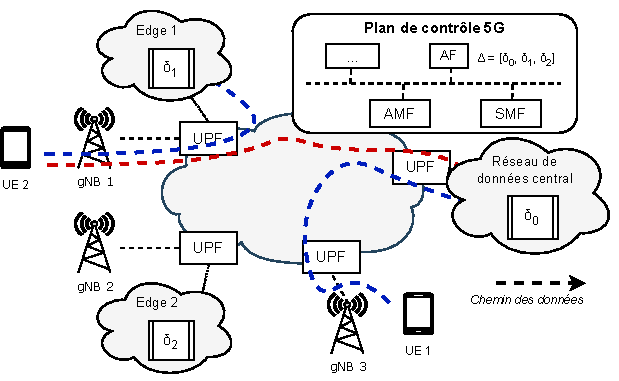
\includegraphics[width=0.85\linewidth]{figs/context-5G-edge.drawio.pdf}
    \caption[\textit{Edge computing} dans un contexte 5G]{Les \gl{UE}{UEs} accèdent à différentes instances ($\delta_0$, $\delta_1$, et $\delta_2$), selon un ensemble de règles que nous allons formaliser.}
    \label{fig:context-5G-edge}
\end{figure}
% Décomposition du problème
Comme indiqué dans la \hyperref[sec:edge-computing]{section~\ref*{sec:edge-computing} du premier chapitre}, le paradigme de l’\textit{edge computing} consiste à déployer au sein du réseau plusieurs \gl{service/instances}{instances des services} disponibles, afin de permettre aux \gl{user}{utilisateurs} d’utiliser les \gl{service/instances}{instances de ces services} qui sont les plus pertinentes au moment où elles sont utilisées.
Par exemple, un des critères utilisés peut être la proximité géographique entre l’\gl{user}{utilisateur} et les \gl{service/instances}{instances}: on va chercher à minimiser la distance afin de réduire la latence.
On peut décomposer ce processus en 3~parties: la gestion du cycle de vie des \gl{service/instances}{instances} (déployer, migrer et supprimer les \gl{service/instances}{instances} en fonction du contexte), la mise en relation (déterminer quelle \gl{service/instances}{instance} doit être utilisée par quel \gl{user}{utilisateur} à quel moment, en suivant une politique pré-établie), et l’accès (permettre à tout instant à l’\gl{user}{utilisateur} d’accéder aux \gl{service/instances}{instances} avec lesquelles il est en relation sans interruption de service).
Nous nous focaliserons dans le cadre de ce manuscrit sur la mise en relation et l’accès.

Nous souhaitons distribuer plusieurs \gl{service/instances}{instances de services}, réparties entre différents \gl{edge}{\textit{edges}}, comme représenté sur la figure~\ref{fig:context-5G-edge}.
Nous avions constaté dans le \hyperref[ch:state-of-the-art]{chapitre précédent} que les solutions existantes pour intégrer l’\textit{edge} dans la 5G ne respectaient pas la totalité de nos exigences, et nous proposons donc SR4MEC, la nouvelle architecture que nous avons conçu dans cette optique.

Nous décomposons notre problème en plusieurs parties, représentées sur la figure~\ref{fig:edges-services-integration-chapter-plan}.

\begin{figure}[h]
    \centering
    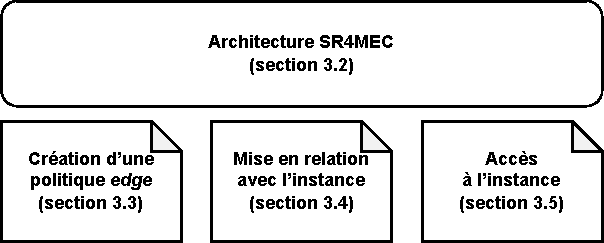
\includegraphics[width=0.62\linewidth]{figs/chapter-plan.drawio.pdf}
    \captionsetup{singlelinecheck=off}
    \caption[]{Pour le cas d’utilisateurs statiques, l’utilisation de services~\textit{edge} pose 3~grandes questions:
    \begin{enumerate}[label=\alph*)]
        \item Comment un opérateur effectue le choix d’une \gl{service/instances}{instance d’un service} pour une \gl{PDU Session}{session~PDU}~?
        \item Comment mettre en relation un équipement utilisateur et \gl{service/instances}{l’instance d’un service}~?
        \item Comment permettre à l’équipement d’accéder à cette \gl{service/instances}{instance}~?
    \end{enumerate}}
    \label{fig:edges-services-integration-chapter-plan}
\end{figure}

Dans un premier temps, nous créons un formalisme qui permettra d’exprimer les critères pour mettre en relation un utilisateur et un \gl{edge}{\textit{edge}} à utiliser.
Nous avons vu dans la \hyperref[sec:placement-instances]{section~\ref*{sec:placement-instances} du chapitre précédent} que les travaux relatifs au problème du placement des \gl{service/instances}{instances} existent en abondance dans la littérature.
Nous proposons donc une abstraction qui nous permettra de ne pas dépendre d’une méthode de placement en particulier, en supposant que cette phase de placement a déjà eu lieu.

Puis, nous montrerons une méthode de distribution de ces règles interopérable avec le système~5G existant, et qui permet leur mise à jour immédiate suite à des événements.
Les solutions existantes ne permettaient pas à la fois le \gl{scalability}{passage à l’échelle} et le contrôle en temps réel par l’opérateur, qui est pourtant indispensable pour changer d’instance dynamiquement et sans interruption de service.

Et enfin, nous verrons comment appliquer ces règles pour mettre en place l’accès effectif au service à travers l’\gl{service/instances}{instance} sélectionnée.

\pagebreak
\section{Aperçu de l’architecture proposée SR4MEC}
\subsection{Séparation des identifiants de services et d’instances}
Afin de permettre aux \gl{UE}{équipements utilisateur} d’utiliser des \gl{service/instances}{services} sans connaître l’identifiant d’une \gl{service/instances}{instance} en particulier, nous prennons inspiration sur \gl{LISP}{LISP} et déléguons la responsabilité du choix de l’instance aux routeurs de bordure.

Nous avions vu dans la \hyperref[sec:LISP]{section~\ref*{sec:LISP} du chapitre précédent} que \gl{LISP}{LISP} n’étant pas prévu pour faire de l’\textit{edge computing}, il n’était pas possible d’avoir une sélection individualisée de l’\gl{service/instances}{instance} pour les \gl{UE}{équipements} d’un même \gl{edge}{\textit{edge}}.

\vspace{1.5cm}
\begin{figure}[h]
    \centering
    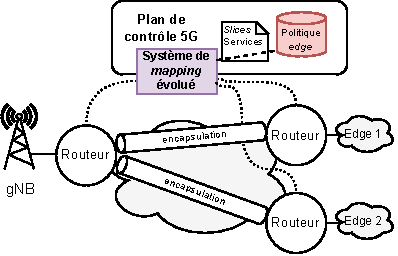
\includegraphics[width=0.7\linewidth]{figs/separation-id-service-instances.drawio.pdf}
    \caption[Séparation des identifiants de services et d’instances dans SR4MEC]{Avec notre système de \textit{mapping} évolué, la \gl{gNB}{gNB} est en mesure d’échanger simultanément des \gl{PDU}{PDUs} avec plusieurs \gl{service/instances}{instances} d’un même \gl{service/instances}{service} chacune située sur un \gl{edge}{\textit{edge}} différent.}
    \label{fig:separation-id-service-instances}
\end{figure}
\vspace{1.5cm}

Nous avons donc besoin d’un système de \textit{mapping} plus évolué que celui de \gl{LISP}{LISP}, capable de récupérer des informations du \gl{CN}{cœur de réseau 5G} afin de répondre de manière différente selon la \gl{PDU Session}{session~PDU}.
Ce système, représenté sur la figure~\ref{fig:separation-id-service-instances}, sera géré par l’opérateur, ce qui lui permettre d’avoir un contrôle total sur la mise en relation.


\pagebreak
\subsection{Abstraction \textit{One Big UPF}}
\label{sec:SR4MEC-One-Big-Upf}
Afin de récupérer les informations nécessaires à notre système de \textit{mapping}, il est nécessaire de communiquer avec le \gl{CN}{cœur de réseau}.
Nous avions vu que certaines approches consistaient à utiliser une \gl{AF}{AF} pour faire cette interface, mais nous ne pourrons pas résoudre le problème du passage à l’échelle tant que nous ne modifierons pas en profondeur la méthode de distribution des règles de routage.
Pour être compatible avec les réseaux~5G existants, nous ne pouvons pas nous permettre de modifier le \gl{SMF}{SMF}, qui est responsable de la distribution des règles.

Nous utilisons donc l’abstraction \textit{One Big UPF}~\cite{10.1145/3482898.3483358}, une variante de l’abstraction \textit{One Big Switch}~\cite{10.1145/2535372.2535373} issue du paradigme \gl{SDN}{SDN}.
Cette abstraction consiste à présenter au \gl{SMF}{SMF} l’ensemble du \gl{CUPS}{plan de données} comme un \gl{UPF}{UPF} unique.

\begin{figure}[h]
    \centering
    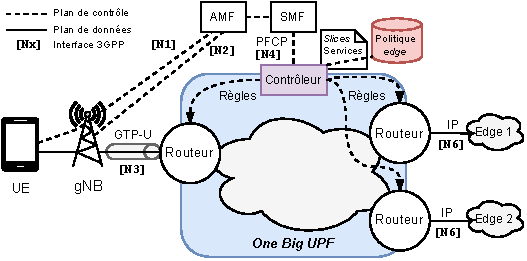
\includegraphics[width=0.85\linewidth]{figs/one-big-upf.drawio.pdf}
    \caption[Abstraction \textit{One Big UPF} dans SR4MEC]{Dans l’abstraction \textit{One Big UPF}, le \gl{SMF}{SMF} n’a plus qu’un seul \gl{UPF}{UPF} à gérer. L’ensemble des informations pertinentes est récupéré par le \gl{controller}{contrôleur} via une interface existante, et il n’est ainsi pas nécessaire de modifier le reste du \gl{CN}{cœur de réseau}.}
    \label{fig:one-big-upf}
\end{figure}

Comme illustré par la figure~\ref{fig:one-big-upf}, notre \textit{Big UPF} est constitué d’un \gl{controller}{contrôleur} et d’un ensemble de routeurs qu’il configure via son interface sud.
Le \gl{controller}{contrôleur} utilise son interface \gl{PFCP}{PFCP} pour communiquer avec le \gl{SMF}{SMF}, si bien que le \gl{SMF}{SMF} le considère comme un \gl{UPF}{UPF} classique.
Le \gl{controller}{contrôleur} connaît à la fois les \gl{UE}{équipements utilisateur} présents sur le réseau, et les \gl{service/instances}{services} qui disposent d’\gl{service/instances}{instances} sur des \gl{edge}{\textit{edges}}.

Cette abstraction réduit grandement le travail du \gl{SMF}{SMF}, puisqu’il n’a plus besoin de maintenir l’ensemble des chemins entre les \gl{UE}{équipements utilisateur} et les \gl{service/instances}{instances de services}.
Elle nous permet à la fois d’utiliser un \gl{controller}{contrôleur~SDN} pour configurer le \gl{CUPS}{plan de données}, et d’utiliser un autre protocole que \gl{GTP}{GTP} pour encapsuler les \gl{PDU}{PDUs}.


\pagebreak
\subsection{Routage par segments}
Pour permettre le passage à l’échelle dans la distribution des règles de routage, nous utilisons du routage par segment.

Grâce à cette méthode que nous avions décrite dans la \hyperref[sec:segment-routing]{section~\ref*{sec:segment-routing} du chapitre précédent}, il est possible pour l’opérateur de contrôler finement les routes utilisées par les \gl{UE}{équipements utilisateurs} pour accéder à des applications~\textit{edge}, tout en réduisant la complexité au sein du réseau (en~réduisant les états à maintenir par le \gl{CN}{cœur de réseau}).

\begin{figure}[h]
    \centering
    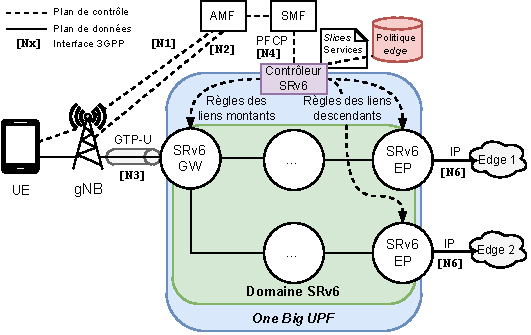
\includegraphics[width=0.85\linewidth]{figs/routage-par-segments.drawio.pdf}
    \caption[Routage par segments dans SR4MEC]{En ajoutant le routage par segments à notre architecture, seuls les nœuds en bordure du réseau doivent être configurés par notre \gl{controller}{contrôleur}: il n’est plus nécessaire de configurer les nœuds intermédiaires du chemin.}
    \label{fig:routage-par-segments}
\end{figure}

Comme illustré sur la figure~\ref{fig:routage-par-segments}, cette technologie nous permet de mettre à jour les chemins de manière immédiate en cas de changement d’\gl{service/instances}{instance} puisque seuls deux nœuds sont configurés par chemin: la \textit{gateway}~SRv6 (SRv6~GW) pour le lien montant, et l’\textit{endpoint}~SRv6 (SRv6~EP) pour le lien descendant.

De plus, il est possible d’ajouter autant de nœuds intermédiaires que désirés tout en épargnant au plan de contrôle la gestion de tunnels, ce qui permet un \gl{scalability}{passage à l’échelle}. 

Nous nous servons en particulier des nouveaux comportements \gl{SRv6}{SRv6} pour le plan utilisateur des réseaux mobiles afin d’obtenir une interopérabilité avec les \gl{gNB}{gNBs} existantes.
Cette partie sera détaillée dans la section~\ref{sec:sr4mec-access} relative au \gl{CUPS}{plan de contrôle et plan de données} pour l’accès à une \gl{service/instances}{instance} spécifique.

\pagebreak
\section{Création d’une politique~\textit{edge}}
\label{sec:edge-policy}
La politique~\textit{edge} prend la forme d’une nouvelle \gl{NF}{fonction} qui peut être interrogée par le \gl{controller}{contrôleur}~\gl{SRv6} dans l’objectif de lier une \gl{PDU Session}{session~PDU} à une \gl{service/instances}{instance d’un service}~\textit{edge}.
Elle est définie par l’opérateur et peut être mise à jour dynamiquement (cf. figure~\ref{fig:edge-policy-general}), par exemple lorsque une nouvelle instance d’une application est créée, suite à la migration d’une instance, ou suite à la suppression d’une instance. 

Pour établir la politique, l’opérateur collabore avec les fournisseurs de services qui peuvent fournir des informations telles que la charge des instances ou encore la consommation d’énergie.
Ces fournisseurs de services peuvent également indiquer des contraintes applicatives (latence, débit, etc.) afin de faciliter la gestion de la \gl{QoS}{qualité de service}.

Les fournisseurs de \gl{service/instances}{services} ne sont pas informés de la localisation de l’équipement utilisateur.
La seule manière pour un fournisseur de service de tenter d’inférer la localisation d’utilisateur est de se fonder sur la localisation de l’instance utilisée (ou vers laquelle une session applicative pré-existante a été migrée), sous réserve que sa sélection se fonde sur des critères exclusivement géographiques, ce qu’il ne peut pas garantir.

\begin{figure}[h]
    \centering
    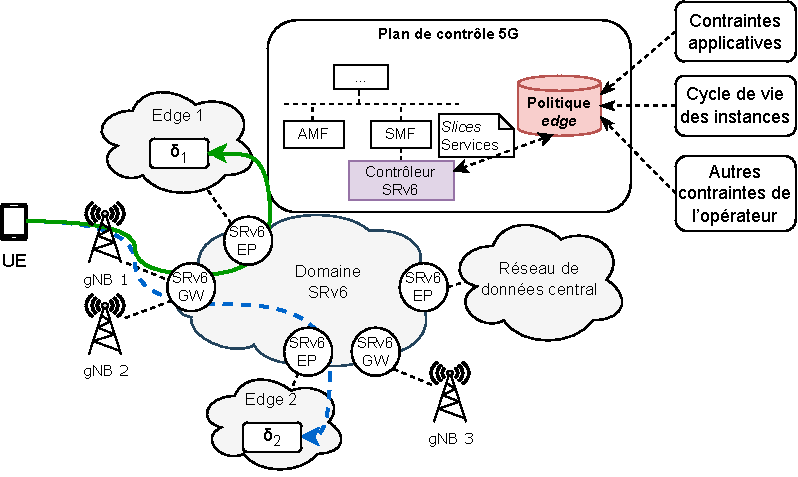
\includegraphics[width=1\linewidth]{figs/edge-policy-general.drawio.pdf}
    \caption[Politiques \textit{edge} dans SR4MEC]{La politique~\textit{edge} met initialement en relation l’\gl{UE}{UE} avec l’instance $\delta_1$. Suite à une évolution de la politique~\textit{edge}, l’\gl{UE}{UE} est mis en relation avec l’instance $\delta_2$.}
    \label{fig:edge-policy-general}
\end{figure}

\subsection{Modélisation d’une politique}
\label{sec:policy-model}
Nous proposons un modèle simplifié de politique~\textit{edge}~(\ref{eq:edge-policy}) où on associera la combinaison d’une \gl{slice}{\textit{slice}}, d’une \textit{area} et d’un \gl{service/instances}{service} à un \gl{edge}{\textit{edge}}.

\begin{equation}
Politique\ Edge: Slice \times Area \times Service \rightarrow Edge
\label{eq:edge-policy}
\end{equation}

Dans notre modèle, pour des raisons de protection de la vie privée et de \gl{scalability}{passage à l’échelle}, la politique~\textit{edge} n’associe pas directement aux \gl{service/instances}{instances}~\textit{edge} une \gl{PDU Session}{session PDU} en particulier, mais des caractéristiques communes de ces dernières.

Une \textit{area} correspond à une étendue géographique depuis laquelle l’\gl{UE}{équipement utilisateur} accède au réseau~5G.
Chaque \textit{area} comprend une \textit{gateway}~\gl{SRv6}{SRv6} et un ensemble de \gl{gNB}{gNBs}.
Une \gl{slice}{\textit{slice}} est une partition du réseau constituée d’un ensemble de ressources, et dédiée à un usage spécifique; elle est identifiée par son \gl{S-NSSAI}{S-NSSAI}.

L’application de cette politique à un \gl{UE}{équipement} est la responsabilité du \gl{controller}{contrôleur}~\gl{SRv6}{SRv6}.
Le \gl{controller}{contrôleur} peut obtenir via d’autres fonctions des informations spécifiques à un \gl{UE}{équipement}, par exemple l’existence de sessions applicatives, l’anticipation d’une mobilité, etc.
Ces informations complémentaires permettent au \gl{controller}{contrôleur} de prendre la meilleure décision pour chaque cas spécifique.

Par la suite, et afin de faciliter les représentations, nous n’étudierons qu’une seule \gl{slice}{\textit{slice}} du \gl{CUPS}{plan de données} à la fois.
Cependant chaque \gl{slice}{\textit{slice}} correspond à un ensemble particulier de ressources, et la politique~\textit{edge} est donc différente en fonction de la \gl{slice}{\textit{slice}} à laquelle accède l’utilisateur.

Dans le cadre de notre modèle, nous considérons qu’il n’y a qu’une seule \gl{service/instances}{instance} d’un même \gl{service/instances}{service} par \gl{edge}{\textit{edge}}.
Nous verrons dans la section~\ref{sec:sr4mec-access} que cette hypothèse de travail permet d’utiliser des \gl{service/instances}{instances} dépourvues de pile~IPv6.
Cependant, lorsque les \gl{service/instances}{instances} ont une double pile~IP (IPv4 et IPv6) on pourra faire évoluer le modèle pour que la politique précise l’identifiant d’une instance particulière~(\ref{eq:edge-policy-instance}).

\begin{equation}
Politique\ Edge: Slice \times Area \times Service \rightarrow (Edge, Instance)
\label{eq:edge-policy-instance}
\end{equation}

\pagebreak
\subsection{Exemples de politiques}
Afin de conserver la possibilité d’accéder à des services \textit{cloud} classiques, accessibles dans le \gl{DN}{réseau de données} central et qui ne sont pas connus par le \gl{CUPS}{cœur de réseau}~5G, on pourra préciser une politique par défaut, comme illustré par la figure~\ref{fig:edge-policy-default}.

Il est éventuellement possible de définir plusieurs règles distinctes par \gl{slice}{\textit{slice}} ou par \textit{area} afin d’équilibrer le trafic entre plusieurs \textit{endpoints}~\gl{SRv6}{SRv6}.

\begin{figure}[h]
    \centering
    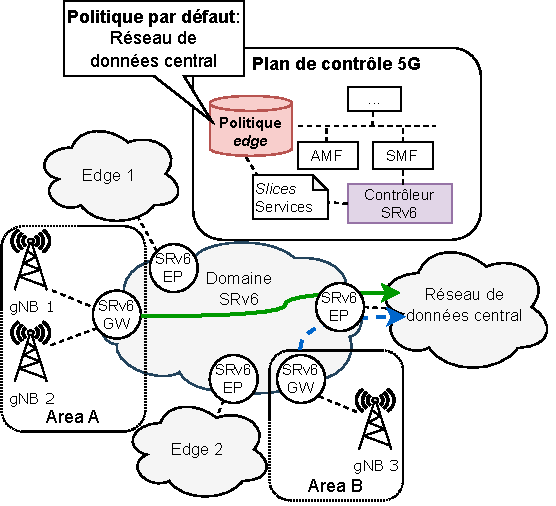
\includegraphics[width=0.85\linewidth]{figs/edge-policy-default.drawio.pdf}
    \caption[]{Lorsque aucune règle plus précise n’a été définie, la politique par défaut consiste à diriger tout le trafic vers le \gl{DN}{réseau de données} central.}
    \label{fig:edge-policy-default}
\end{figure}

\pagebreak

Dans le cas de services~\textit{edge}, il est possible de diriger le trafic vers un \gl{edge}{\textit{edge}} en particulier selon des critères définis par l’opérateur.
Pour des services d’infrastructure essentiels comme des résolveurs~\gl{DNS}{DNS}, l’opérateur fera probablement le choix de déployer une instance de ce service par \gl{edge}{\textit{edge}} et de systématiquement diriger le trafic vers l’\gl{edge}{\textit{edge}} le plus proche.

Au contraire, certains \gl{service/instances}{services} peuvent n’être disponibles que dans certains~\gl{edge}{\textit{edges}} (voir la figure~\ref{fig:edge-policy-by-area-service}).
\begin{figure}[h]
    \centering
    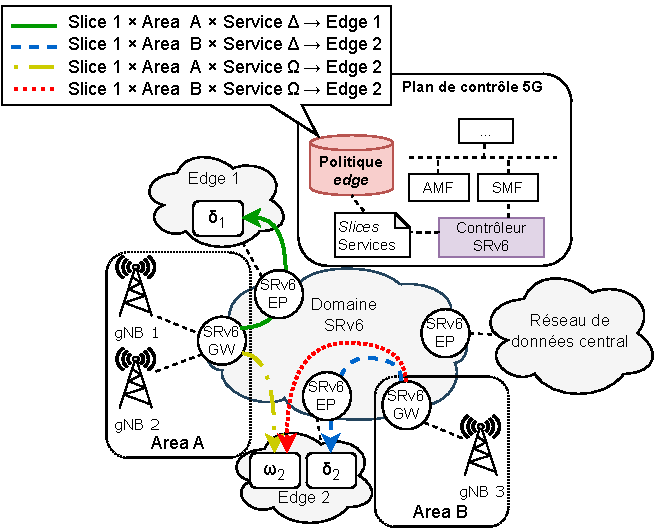
\includegraphics[width=0.85\linewidth]{figs/edge-policy-by-area-service.drawio.pdf}
    \caption[]{Le service $\Delta$ est un service d’infrastructure déployé dans tous les \gl{edge}{\textit{edges}}. La politique~\textit{edge} a été définie de manière a associer chaque \textit{area} à l’\gl{edge}{\textit{edge}} le plus proche pour ce service. Le service $\Omega$ n’est déployé que dans l’\gl{edge}{\textit{edge}}~2: les deux \textit{areas} accèdent donc à l’instance $\omega_2$.}
    \label{fig:edge-policy-by-area-service}
\end{figure}
\pagebreak

\section{Mise en relation avec une instance}
La mise en relation est l’étape qui consiste à associer une \gl{PDU Session}{session~PDU} à une \gl{service/instances}{instance}~\textit{edge}. Cette étape peut être initiée à divers instants clés, illustrés par la figure~\ref{fig:chronologie-mise-en-relation}, tout le long de la vie d’une \gl{PDU Session}{session~PDU}.

\begin{figure}[h]
    \centering
    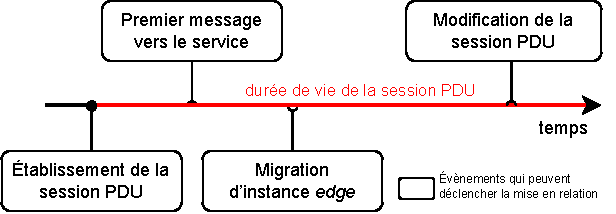
\includegraphics[width=0.9\linewidth]{figs/chronologie-mise-en-relation.drawio.pdf}
    \caption[Mise en relation avec une instance dans SR4MEC]{La mise en relation peut être s’effectuer en réaction à des évènements tout le long de la vie de la \gl{PDU Session}{session PDU}, ou pro-activement dès son établissement.}
    \label{fig:chronologie-mise-en-relation}
\end{figure}

De manière générale, on souhaitera anticiper les accès afin de mettre en relation aussi tôt que possible, mais on devra trouver un compromis qui limite le nombre de relations à maintenir.

Pour les \gl{service/instances}{services} d’infrastructure essentiels, on cherchera généralement à faire la mise en relation dès l’établissement de la \gl{PDU Session}{session~PDU} pour réduire le temps de transmission de la première \gl{PDU}{PDU}.
Chaque \gl{slice}{\textit{slices}}, peut définir un groupe différent de services essentiels: par exemple, pour des \gl{slice}{\textit{slices}} \gl{IoT}{IoT}, \gl{V2X}{V2X} ou \gl{eMBB}{eMBB}, les usages sont différents et les services essentiels seront le reflet de cette diversité.

Les autres \gl{service/instances}{services}~\textit{edge} sont plus nombreux, et on ne seront pas obligatoirement utilisés par l’\gl{UE}{équipement}.
Il serait très coûteux pour le \gl{CUPS}{plan de contrôle} de mettre en relation chaque utilisateur avec une instance de chaque service disponible, et de maintenir autant de relations alors que seule une fraction d’entre-elles seront utilisées.
C’est pourquoi il est possible d’utiliser un mode réactif: pour cet ensemble de services~\textit{edge} on effectuera la mise en relation lors de l’émission par l’\gl{UE}{équipement utilisateur} de la première \gl{PDU}{PDU}.

À chaque instant, il est possible de faire une migration d’\gl{service/instances}{instance}~\textit{edge}, qui viendra donc modifier la mise en relation.
Une autre stratégie réactive peut ainsi consister à utiliser dans un premier temps le \gl{DN}{réseau de données} central, et à ne migrer vers un \gl{edge}{\textit{edge}} que dans un second temps.

Lors de la modification ou la libération de la \gl{PDU Session}{session~PDU}, on pourra également mettre à jour les relations, ou les sauvegarder dans le \gl{CUPS}{plan de contrôle} en prévision d’une mobilité.
\pagebreak

\subsection{Application de la politique~\textit{edge}}
La liste des \gl{service/instances}{services} à configurer pour une \gl{PDU Session}{session} dépendra de la politique~\textit{edge}.
Pour être en mesure de l’appliquer, le \gl{controller}{contrôleur}~\gl{SRv6}{SRv6} doit déterminer dans quelle \textit{area} se situe l’\gl{UE}{équipement utilisateur} et sur quelle \gl{slice}{\textit{slice}} s’établit cette \gl{PDU Session}{session}.
Ces informations sont récupérées par l’interface~\gl{PFCP}{PFCP} lors de l’établissement ou de la modification de la \gl{PDU Session}{session PDU} (voir figure~\ref{fig:application-politique-edge}).

\begin{figure}[h]
    \centering
    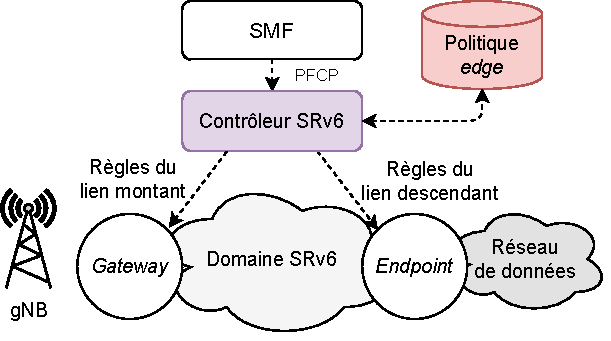
\includegraphics[width=0.6\linewidth]{figs/application-politique-edge.drawio.pdf}
    \caption[Application des politiques \textit{edge} par SR4MEC]{Lors de l’établissement d’une nouvelle \gl{PDU Session}{session~PDU}, le contrôleur \gl{SRv6}{SRv6} reçoit des règles~\gl{PFCP}{PFCP} sur son interface nord.}
    \label{fig:application-politique-edge}
\end{figure}

Pour chaque \gl{PDU Session}{session~PDU}, il est également nécessaire de connaître à la fois les \gl{TEID}{identifiants des deux tunnels GTP} utilisés (pour le lien montant et le lien descendant), ainsi que l’adresse~IP de la \gl{gNB}{gNB} (pour le lien montant).
Ces informations serviront à créer des chemins de bout-en-bout entre l’\gl{UE}{équipement} et l’\gl{edge}{\textit{edge}}, comme illustré sur la figure~\ref{fig:establishment-procedure}.

\begin{figure}[h]
    \centering
    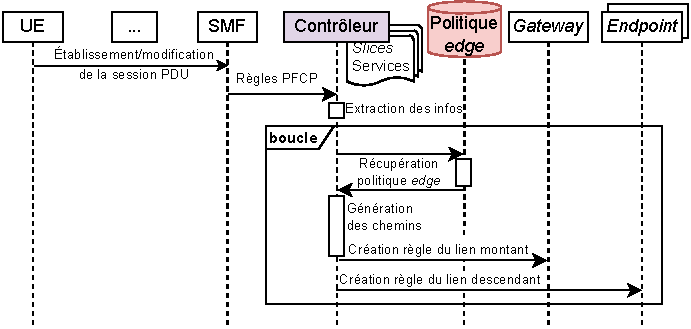
\includegraphics[width=0.8\linewidth]{figs/establishment-procedure.drawio.pdf}
    \caption[Procédure de traduction de règles PFCP par SR4MEC]{Lors de l’établissement de la \gl{PDU Session}{session~PDU}, le \gl{controller}{contrôleur} extrait des informations depuis les règles \gl{PFCP}{PFCP} configurées par le \gl{SMF}{SMF}. Il se sert de ces informations pour appliquer la politique~\textit{edge} et générer les chemins de données pour la \gl{PDU Session}{session~PDU}.}
    \label{fig:establishment-procedure}
\end{figure}

Lorsqu’une \gl{PDU Session}{session~PDU} est établie, le \gl{SMF}{SMF} configure notre \textit{Big UPF} avec deux jeux de règles qui sont créées au sein d’une session~\gl{PFCP}{PFCP}.
Le standard~5G ne garantit aucune équivalence entre une \gl{PDU Session}{session~PDU} et une session \gl{PFCP}{PFCP}, même si une telle équivalence facilite la gestion des sessions pour le~\gl{SMF}{SMF}.
Selon l’implémentation, il est possible d’utiliser une session~\gl{PFCP}{PFCP} pour plusieurs \gl{PDU Session}{sessions~PDU}: la session~\gl{PFCP}{PFCP} regroupe alors des règles pour la gestion des tunnels~\gl{GTP}{GTP} de toutes les \gl{PDU Session}{sessions~PDU} configurées sur cette session \gl{PFCP}{PFCP}.
Il devient alors possible pour le \gl{SMF}{SMF} de configurer plusieurs \gl{PDU Session}{sessions PDU} au sein d’un unique message~\gl{PFCP}{PFCP}.
À l’inverse, même si les règles du lien montant et du lien descendant appartiennent toujours à la même session~\gl{PFCP}{PFCP}, rien n’impose au \gl{SMF}{SMF} de les configurer au moyen d’un seul message~\gl{PFCP}{PFCP}.
Aussi, pour récupérer les informations dont nous avons besoin, nous ne pouvons nous fier ni à la notion de session~\gl{PFCP}{PFCP}, ni à la co-occurrence de règles au sein d’un message~\gl{PFCP}{PFCP}, ce qui nous amène à considérer les règles émanant du \gl{SMF}{SMF} de manière individuelle.

Dans un premier temps, nous souhaitons associer chaque règle à une \gl{slice}{\textit{slice}} car c’est le premier paramètre de notre politique~\textit{edge}.
Le \gl{S-NSSAI}{S-NSSAI} n’est pas directement transmit dans les règles~\gl{PFCP}{PFCP}, il faudra donc se baser sur l’adresse~IP qui a été attribuée à la \gl{PDU Session}{session~PDU} et déduire la \gl{slice}{\textit{slice}} de cette information, par exemple en définissant des plages d’adresses~IP différentes pour chaque \gl{slice}{\textit{slice}}.
\gl{PFCP}{PFCP} propose un champ « adresse~IP de l’\gl{UE}{UE} » qui contient cette information.
Ce champ est obligatoire pour les règles du lien descendant, mais pas pour le lien montant.
Cependant, il est nécessaire à la fois pour gérer la \gl{QoS}{qualité de service} et la facturation, nous considérons donc que ce champ sera toujours présent.

\begin{figure}[h]
    \centering
    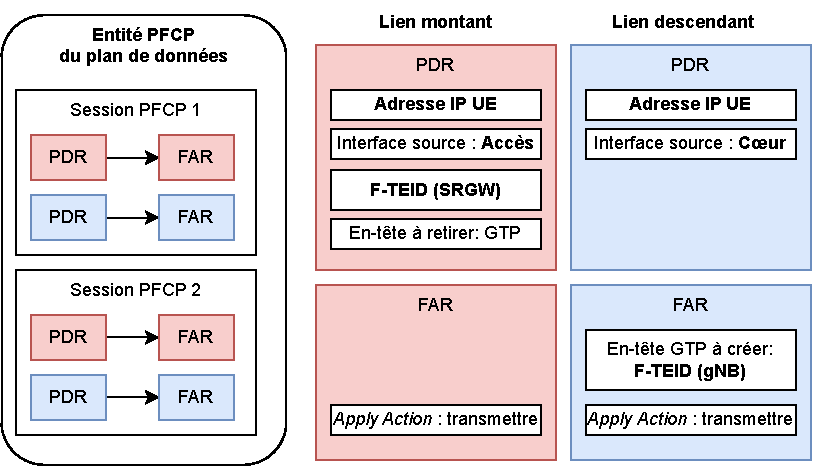
\includegraphics[width=0.9\linewidth]{figs/pfcp-rules-one-big-upf.drawio.pdf}
    \caption[Contenu des règles PFCP de la 5G]{Dans notre architecture, le \textit{Big \gl{UPF}{UPF}} reçoit des règles~\gl{PFCP}{PFCP} qui permettent de faire le lien entre la \gl{gNB}{gNB} et le \gl{DN}{réseau de données}. Il n’y a qu’un seul \gl{UPF}{UPF}, donc il n’y a pas de règle de chaînage de tunnels. Pour chaque \gl{PDU Session}{session~PDU}, deux ensembles de règles sont créés. Chaque ensemble est constitué d’une \gl{PDR}{\textit{Packet Detection Rule} (PDR)} qui est associée à une \gl{FAR}{\textit{Forwarding Action Rule} (FAR)}.}
    \label{fig:pfcp-rules-one-big-upf}
\end{figure}

\pagebreak

Nous pouvons identifier le sens du lien grâce au champ « interface source » de la règle~\gl{PFCP}{PFCP}: les \gl{PDU}{PDUs} en provenance du \gl{RAN}{réseau d’accès} sont associées au lien montant, et celles qui viennent du \gl{CN}{cœur de réseau} au lien descendant.

Comme représenté sur la figure~\ref{fig:pfcp-rules-one-big-upf}, le \gl{F-TEID}{F-TEID (\textit{Fully Qualified Tunnel Endpoint Identifier})} contenu dans la règle du lien montant correspond au \gl{TEID}{numéro de tunnel} sur lequel la \textit{gateway} doit écouter ainsi que l’adresse~IP de la \textit{gateway}.
L’adresse~IP de la \gl{gNB}{gNB} n’est pas contenue dans cette règle, mais il n’est pas nécessaire de la connaître pour configurer une première règle de routage~\gl{SRv6} pour le lien montant; nous avons uniquement besoin de connaître l’\textit{area} dans laquelle se situe l’\gl{UE}{équipement utilisateur}.

Pour le lien descendant, le \gl{F-TEID}{F-TEID} correspond au \gl{TEID}{numéro de tunnel} à utiliser ainsi que de l’adresse~IP de la \gl{gNB}{gNB}.
Pour constituer le chemin descendant, il est également nécessaire de savoir dans quelle \textit{area} est située cette \gl{gNB}{gNB}.
Si cette information n’est pas préalablement connue par le \gl{controller}{contrôleur}, il est possible de rassembler les paires de règles \gl{PFCP}{PFCP} montantes et descendantes pour obtenir l’adresse de la \textit{gateway} qui est contenue dans le \gl{F-TEID}{F-TEID} de la règle~\gl{PFCP}{PFCP} du lien montant.

En associant chaque \textit{area} à une \textit{gateway} différente, comme illustré sur la figure~\ref{fig:pfcp-one-big-upf}, nous pouvons déduire cette dernière information manquante de l’adresse~IP de la \textit{gateway}.
Nous verrons dans le \hyperref[ch:mobility]{chapitre suivant} que l’utilisation d’une \textit{gateway} différente pour chaque \textit{area} joue un rôle important pour les scénarios de mobilité.

\begin{figure}[h]
    \centering
    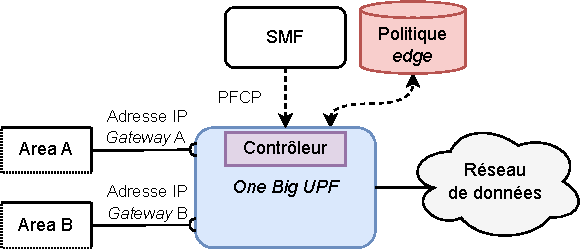
\includegraphics[width=0.85\linewidth]{figs/pfcp-one-big-upf.drawio.pdf}
    \caption[Gestion des zones géographiques par SR4MEC]{Chaque \textit{area} utilise une \textit{gateway} différente, munie d’une adresse~IP distincte. Du point de vue du \gl{CUPS}{plan de contrôle}, chaque \textit{gateway} constitue une interface~\gl{GTP}{GTP} du \textit{Big~\gl{UPF}{UPF}}.}
    \label{fig:pfcp-one-big-upf}
\end{figure}

\pagebreak

\subsection{Changement d’instance~\textit{edge}}
\label{sec:edge-instance-rebinding}
Dans le cas d’un changement d’\gl{service/instances}{instance}, on voudra s’assurer qu’aucune \gl{PDU}{PDU} ne se perde.
En utilisant la procédure décrite sur la figure~\ref{fig:edge-instance-rebinding-procedure}, il est possible de garantir qu’à tout instant il existe un chemin valide entre l’équipement et une \gl{service/instances}{instance du service}.

\vspace{1.5cm}
\begin{figure}[h]
    \centering
    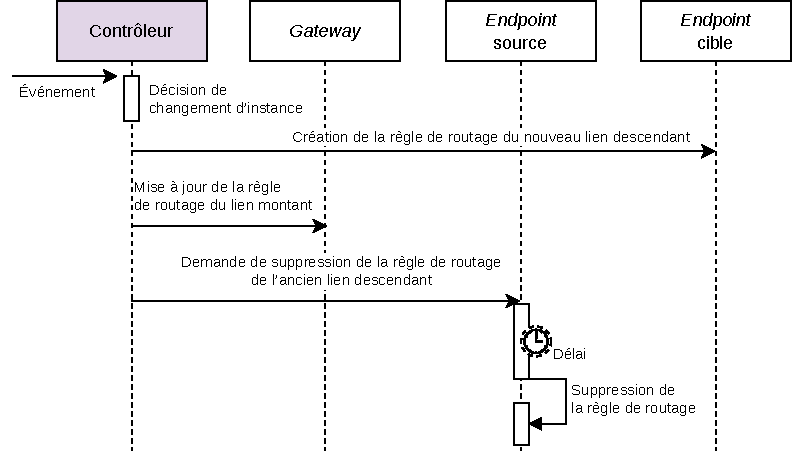
\includegraphics[width=0.95\linewidth]{figs/edge-instance-rebinding-procedure.drawio.pdf}
    \caption[Procédure de changement d’instance par SR4MEC]{Le changement d’\gl{service/instances}{instance} s’effectue de manière transparente pour l’\gl{user}{utilisateur}. La \gl{PDU Session}{session~PDU} n’est pas modifiée, et les routes sont maintenues de manière à ne perdre aucune \gl{PDU}{PDU}.}
    \label{fig:edge-instance-rebinding-procedure}
\end{figure}
\vspace{1.5cm}

Dans un premier temps, il est nécessaire de créer une route entre l’\gl{service/instances}{instance} cible et l’\gl{UE}{utilisateur} pour le lien descendant sur l’\textit{endpoint} de l’\gl{edge}{\textit{edge}} cible.
Lorsque l’\gl{service/instances}{instance} cible est prête à répondre aux messages de l’\gl{UE}{équipement utilisateur}, le chemin configuré sur le lien montant existant peut être mis à jour dans la \textit{gateway} afin de diriger vers l’\gl{service/instances}{instance} cible.

Dès que la nouvelle route est configurée, les \gl{PDU}{PDUs} nouvellement émises seront reçues par la nouvelle \gl{service/instances}{instance}.
Cependant, l’\gl{service/instances}{instance} source est encore susceptible de recevoir des \gl{PDU}{PDUs} en cours d’acheminement ou de traitement.
On devra donc attendre l’écoulement d’un délai suffisant avant de supprimer l’ancienne route sur l’\textit{endpoint} source.


\section{Accès à l’instance}
\label{sec:sr4mec-access}
Lors de la mise en relation, le \gl{controller}{contrôleur}~\gl{SRv6}{SRv6} provisionne des règles \textit{match-action} en bordure du domaine~\gl{SRv6}{SRv6}.
Il convient ensuite de raffiner ces règles pour le \gl{CUPS}{plan de données} selon l’approche « SRv6 pour le plan utilisateur des réseaux mobiles »~\cite{rfc9433} présentée dans la \hyperref[sec:SRv6-MUP]{section~\ref*{sec:SRv6-MUP} du chapitre précédent}.

Une première règle est envoyée sur la \textit{gateway} pour le créer le lien montant.
La SRGW implémente le comportement~\gl{SRv6}{SRv6} \texttt{H.M.GTP4.D}, et associe un \gl{TEID}{TEID} à un ensemble de segments~\gl{SRv6} qui forment le chemin du lien montant.

Comme illustré sur la figure~\ref{fig:access-to-instance}, toutes les informations présentes dans l’en-tête~\gl{GTP}{GTP} sont encodées dans l’en-tête~IPv6 et le \gl{SRH}{\textit{Segment Routing Header} (SRH)}.
Ces informations incluent en particulier le \gl{TEID}{TEID} (32~bits), le champ QFI (\textit{\gl{QoS}{QoS} Flow Identifier}, 6~bits).
Certaines de ces informations ne sont cependant pas essentielles pour notre architecture puisqu’une fois entrée dans le domaine~\gl{SRv6}{SRv6} nous ne ré-encapsulons pas la \gl{PDU}{PDU} dans un tunnel~\gl{GTP}{GTP}.
En effet, le nœud de sortie du domaine implémente le comportement \texttt{End.DX4} (dés-encapsulation et interconnexion avec IPv4), ce qui permet une compatibilité avec un \gl{edge}{\textit{edge}} en IPv4.
Si on souhaite modifier l’architecture pour proposer plusieurs \gl{service/instances}{instances} d’un même \gl{service/instances}{service} au sein d’un même \gl{edge}{\textit{edge}}, il faudra implémenter la fonction de sortie du domaine directement sur l’\gl{service/instances}{instance}.

\begin{figure}[h]
    \centering
    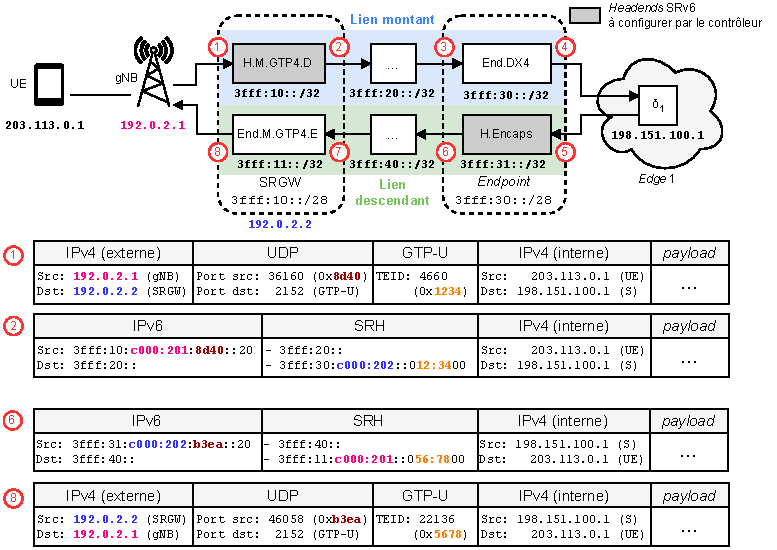
\includegraphics[width=0.95\linewidth]{figs/access-to-instance.drawio.pdf}
    \caption[Format des paquets SRv6 MUP]{Les \textit{headends} sont configurés par le \gl{controller}{contrôleur}~\gl{SRv6}{SRv6} suivant la politique~\textit{edge}. La SRGW fait la correspondance entre les en-têtes \gl{GTP}{GTP} et \gl{SRv6}{SRv6}.}
    \label{fig:access-to-instance}
\end{figure}
    
Une deuxième règle est envoyée sur l’\textit{endpoint} pour créer le lien descendant. 
L’\textit{endpoint} associe l’adresse~IP de destination (c’est-à-dire l’adresse de l’\gl{UE}{équipement utilisateur}) à un second ensemble de segments qui forment le chemin du lien descendant.
Il est cette fois nécessaire d’indiquer dans les en-têtes à la fois le \gl{TEID}{numéro de tunnel} et l’adresse~IP de la \gl{gNB}{gNB} à laquelle est connectée l’\gl{UE}{équipement}.
De la même manière que pour le lien montant, nous encodons l’adresse~IPv4 source à utiliser pour le lien~\gl{GTP}{GTP} dans la fin de l’adresse~IPv6 source du paquet.

Pour aider à équilibrer la charge, \gl{GTP}{GTP} prévoit la possibilité d’utiliser plusieurs ports source différents selon l’origine du trafic, nous dévions donc de la proposition initiale de la RFC~9433 pour ajouter cette information au sein des deux octets qui suivent l’encodage de l’adresse~IPv4.
Dans la RFC~9433, tous les bits suivant l’encodage de l’adresse~IPv4 étaient ignorés.

Afin de permettre l’utilisation de préfixes~IPv6 de longueur variable pour les différents segments et de ne pas avoir à conserver cet état dans la SRGW pour tous les \textit{headends} implémentés dans le domaine, nous encodons la longueur du préfixe~IPv6 dans les 7~derniers bits du champs adresse~IPv6 source (voir figure~\ref{fig:ipv6-source-format}).

\begin{figure}[h]
    \centering
    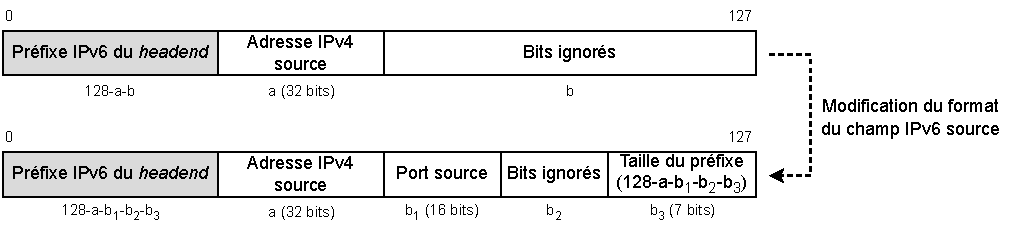
\includegraphics[width=1\linewidth]{figs/IPv6-source-format.drawio.pdf}
    \caption[Encodage d’information dans les adresses IPv6 avec SRv6 MUP]{Nous proposons de modifier l’encodage de l’adresse~IPv6 source pour le comportement \texttt{End.M.GTP4.E} en ajoutant le port~source et la taille du préfixe~IPv6.}
    \label{fig:ipv6-source-format}
\end{figure}

Lorsque l’on encode ces informations supplémentaires dans l’adresse~IPv6 source, il reste 73~bits pour le \textit{locator} et l’identifiant de la fonction ayant créé le paquet initial, ce qui reste supérieur à ce qui est disponible lorsque l’on encode l’adresse du segment final du lien descendant.

\pagebreak
\section{Impact de l’architecture SR4MEC sur le plan de contrôle}
Pour déterminer l’impact de notre architecture sur le \gl{CUPS}{plan de contrôle}, nous pouvons la comparer avec une architecture~5G classique avec des \gl{ULCL}{\textit{Uplink Classifiers} (ULCLs)}.
Dans le tableau~\ref{table:cp-rules}, nous analysons le nombre de sessions à maintenir et le nombre de messages de contrôle requis pour effectuer trois étapes d’un scénario d’\textit{edge computing}.
À l’établissement de la \gl{PDU Session}{session~PDU}, nous configurons l’accès au réseau central: il s’agit de la règle par défaut.
Puis nous appliquons une politique~\textit{edge} pour mettre en relation l’\gl{user}{utilisateur} avec une instance~\textit{edge}.
Et enfin, nous considérons le cas du changement d’\gl{service/instances}{instance}, par exemple suite à la migration de celle-ci vers un autre \gl{edge}{\textit{edge}}.

\begin{table}[h]
\begin{tabular}{l|cc|ccc}
\toprule
 & \multicolumn{2}{c|}{\textbf{\gl{ULCL}{ULCL}}} & \multicolumn{3}{c}{\textbf{SR4MEC}} \\
 & \multicolumn{1}{c}{\textbf{Sessions \gl{PFCP}{PFCP}}} & \multicolumn{1}{c|}{\textbf{\gl{PDR}{PDRs}}} & \multicolumn{1}{c}{\textbf{Sessions \gl{PFCP}{PFCP}}} & \multicolumn{1}{c}{\textbf{\gl{PDR}{PDRs}}} & \multicolumn{1}{c}{\textbf{Règles \gl{SR}{SR}}} \\
\midrule
Accès réseau central                          & $|\mathit{UPF}|$ & $2{\times}|\mathit{UPF}|$ & 1 & 2 & 2 \\
Accès \gl{edge}{réseau \textit{edge}}         & $|\mathit{UPF}|$ & $2{\times}|\mathit{UPF}|$ & 0 & 0 & 2 \\
Changement d’\gl{service/instances}{instance} & $3{+}|\mathit{UPF_I}|$ &  $6{+}2{\times}|\mathit{UPF_I}|$ & 0 & 0 & 3 \\
\bottomrule
\end{tabular}
\caption[Impact de SR4MEC sur le plan de contrôle]{Comparaison du nombre de sessions à maintenir et de messages de contrôle nécessaires par \gl{PDU Session}{session~PDU} pour diriger les données vers différents réseaux, selon l’architecture utilisée: une architecture~5G classique avec des \gl{ULCL}{\textit{Uplink Classifiers}} ou notre architecture SR4MEC.}
\label{table:cp-rules}
\end{table}

Pour l’architecture classique, le nombre de sessions~\gl{PFCP}{PFCP} dépend du nombre d’\gl{UPF}{UPF} ($|\mathit{UPF}|$) dont est formé le chemin de données.
Dans les deux premières étapes, il est nécessaire de configurer chacun des nœuds donc autant de sessions~\gl{PFCP}{PFCP} seront créées ou mises à jour.
Au contraire, dans notre architecture~SR4MEC il n’existe qu’un seul \textit{Big~\gl{UPF}{UPF}}: il n’y a qu’une seule session à créer dans la première étape, et par la suite le \gl{SMF}{SMF} n’a plus de configuration a effectuer puisque c’est le \gl{controller}{contrôleur}~\gl{SRv6}{SRv6} qui est en charge d’appliquer la politique~\textit{edge}, et non le \gl{SMF}{SMF}.

Avec les \gl{ULCL}{ULCLs}, la troisième~étape nécessite de mettre à jour les sessions~\gl{PFCP}{PFCP} sur les nœuds suivants:
\begin{itemize}
    \item le premier \gl{UPF}{UPF} du chemin, qui s’interface avec la \gl{gNB}{gNB};
    \item l’\gl{UPF}{UPF} de l’\gl{edge}{\textit{edge}} source;
    \item l’\gl{UPF}{UPF} de l’\gl{edge}{\textit{edge}} cible;
    \item tous les éventuels autres \gl{UPF}{UPFs} intermédiaires (UPF\textsubscript{I}) qui composent l’ancien et le nouveau chemin.
\end{itemize}
De la même façon que pour la deuxième~étape, aucune session~PFCP n’est impliquée dans la troisième~étape dans notre architecture~SR4MEC.

Dans les trois étapes, puisqu’il est nécessaire de configurer des règles à la fois pour le lien montant et le lien descendant, le nombre de \gl{PDR}{PDRs} à créer, supprimer ou mettre à jour est le double du nombre de sessions~\gl{PFCP}{PFCP} à créer ou mettre à jour.

Dans l’architecture~SR4MEC, le \gl{controller}{contrôleur}~\gl{SRv6}{SRv6} est responsable de la création des chemins.
Il doit donc envoyer des messages de contrôle vers les routeurs situés en bordure du domaine~\gl{SRv6}{SRv6}: il y a donc deux routeurs à configurer pour les accès initiaux à des réseaux, et trois routeurs lors du changement d’\gl{service/instances}{instance~\textit{edge}}.

On remarquera que notre architecture~SR4MEC réduit considérablement la charge de travail du \gl{SMF}{SMF}, et pour ces différentes étapes rend le nombre de messages de contrôle échangés constant et indépendant du nombre de routeurs dans le réseau de transport de l’opérateur.

\section{Synthèse}
Dans ce chapitre, nous avons proposé une architecture permettant d’intégrer des services~\textit{edge} dans des réseaux~5G existants.
Nous avons montré que cette architecture est compatible avec le \gl{CUPS}{plan de contrôle~5G}, et qu’elle réduit le nombre d’états à maintenir et la quantité de messages de contrôle.

Cette architecture est capable de diriger le trafic des \gl{user}{utilisateurs} vers l’\gl{edge}{\textit{edge}} le plus adapté à chaque situation, mais les \gl{service/instances}{services} n’obtiennent pas d’accès à la localisation précise des \gl{user}{utilisateurs}, préservant leur vie privée.
L’opérateur contrôle en temps réel la mise en relation entre l’\gl{user}{utilisateur} et les \gl{service/instances}{instances des services}, et l’architecture permet une migration d’\gl{service/instances}{instance} transparente pour l’\gl{user}{utilisateur}.

Nous avons étudié dans ce chapitre le cas d’utilisateurs statiques.
Nous aborderons la gestion de la mobilité des utilisateurs dans le \hyperref[ch:mobility]{prochain chapitre}, et montrerons comment il est possible de la prendre en compte dans notre architecture.
\end{document}